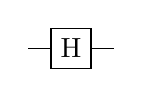
\begin{tikzpicture}[
  baseline=(current bounding box.center),
  x=1em,
  y=1em,
  wire/.style={line width=0.35pt},
  one qubit gate/.style={
    draw,
    line width=0.45pt,
    fill=white,
    minimum width=1.45em,
    minimum height=1.45em,
    inner sep=0pt
  }
]
  \foreach [count=\row from 0] \gateLabel in {H} {
    \pgfmathsetmacro{\y}{-\row * 1.95}
    \draw[wire] (-1.55,\y) -- (1.55,\y);
    \node[one qubit gate] at (0,\y) {$\mathrm{\gateLabel}$};
  }
\end{tikzpicture}
